\chapter{Vehicle Semantics Extraction}

\label{section:semanticsextraction}


\section{Introduction}

This chapter focuses on the first objective [O1] of identifying and extracting suitable semantics that accurately describes vehicle attributes and events within a car park setting. Hence, the implementation of the vehicle semantic extraction module will be discussed in detail.
First, an atom-based quantization process for the video data is introduced in Section~\ref{section:atoms}. This quantization technique was adapted and implemented in both \versionOneExt and \versionTwoExt frameworks. Next, the process of obtaining the vehicle's bounding box is discussed briefly in Section~\ref{subsection:fundamental}.
The following sections thoroughly describes both of the vehicle semantic extraction modules in Section~\ref{section:semantic_lsh} and Section~\ref{section:semantic_chamfer}.

%may be good to add a short paragraph to briefly describe and reinforce what "vehicle semantics extraction" is in relation to the big problem and that two extractions methods are introduced in this research and why two .... along with giving a brief distinction between the two.

As the focus of this work revolves around car park surveillance footage, colour and motion data are key information used to describe vehicle activities. With the goal of designing retrieval techniques suitable for car park surveillance footage, accurate extraction of these information is a crucial component of this work.
%While there are several differences between the two phases of the extraction methods,
Fundamentally, these two phases has the same objective of extracting semantics from the video data.
The predominant difference lies with how the extracted semantics were stored. The flexibility of the outputs produced from the extraction modules affects the performance of the retrieval engine drastically.
The extracted semantics from the \versionOneExt are akin to keywords in a \textit{keyword-based} retrieval system. Hence, the proposed corresponding retrieval technique was placed in a hit-or-miss situation. On the other hand, the \versionTwoExt utilises probability scores to describe the extracted semantics. Hence, increasing the overall robustness of the retrieval engine.



\section{Atom-based Quantization}
\label{section:atoms}

As the utilisation of video data is central to this work, there's an urgent need to come up with a way to easily manipulate and represent the video information. Given that video data can be represented using the 3-dimensional space through \textit{X-axis, Y-axis, \& time-axis}, quantization techniques were applied to convert the continuous data into discrete data blocks.


\begin{figure}[H]\centering
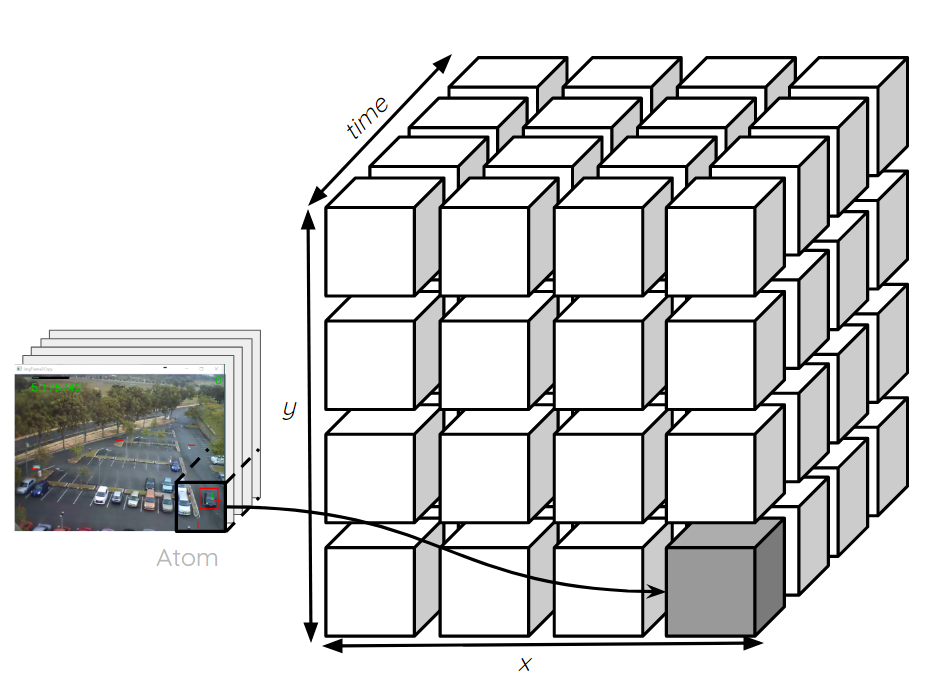
\includegraphics[width=0.6\textwidth]{image/general/atom.PNG}
\caption[Quantization of Video Data into Atoms.]
{Quantization of Video Data into Atoms.
Inspired by the works of \citeA{castanon2016retrieval}.}
\label{fig:atoms}
\end{figure}


%In order to design a framework for long-term vehicle semantics extraction from video data,
This work adopted the concept of \textbf{``atoms''} as coined by \cite{castanon2016retrieval} which enables quantization of the video input into individual 3D spatial-temporal cuboids. In this work, an atom is defined as a group of pixels at a similar spatial location spanning across a fixed number of frames; hence forming a spatio-temporal `cuboid'.
As described in Section~\ref{section:dataset_used}, the video dataset uses a resolution of 640$\times$480 pixels with a frame rate of 10$fps$.
The dimensions of each atom ($\alpha$) is set to $\alpha_{width}=32$ pixels, $\alpha_{height}=24$ pixels and $\alpha_{time}=10$ frames - which represents the temporal duration of 1 second.
The dimensions of the atom ($\alpha_{width},\alpha_{height}$) were set such that the input video data can be uniformly divided by 20 across its width and height as illustrated in Figure~\ref{fig:viewfromcamera}. Using this setup, each atom could be uniquely identified using the $X, Y$ and $T$ identifiers.

Given that the accuracy of data representation relies heavily upon the number of spatio-temporal cuboids used, $\alpha_{width}$ and $\alpha_{height}$ is selected such that one and only one vehicle can occupy a single atom block at any given time. Hence, the colour and trajectory semantics of the vehicles can be adequately represented.
While smaller atoms could be used to accurately capture the exact location of the vehicle, the additional atoms would add towards extra computational power needed to process the queries. This property will be discussed in Chapter~\ref{section:retrievalengine}.

The use of these spatial-temporal cuboids is paramount in this work.
By applying the quantization on all axis, the atom-based structure simplifies the filtering process of two major types of queries.
Figure~\ref{fig:typesofQuery} illustrates the types of queries which are regularly desired when working with video data: \textit{Region of Interest (ROI) query} \& \textit{Time-slicing query}.
Moreover, real-world applications queries typically combines both ROI and time-slicing queries where specific activities which occurred in a particular location within a time frame is desired.


\begin{figure}[htb!]
  \centering
  \begin{tabular}{cc}
  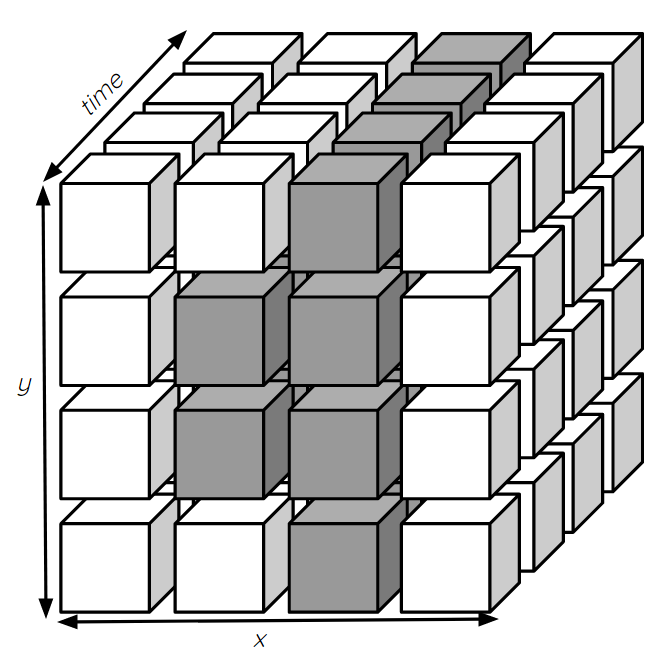
\includegraphics[width=0.3\linewidth]{image/general/atom_ROI.PNG} &
  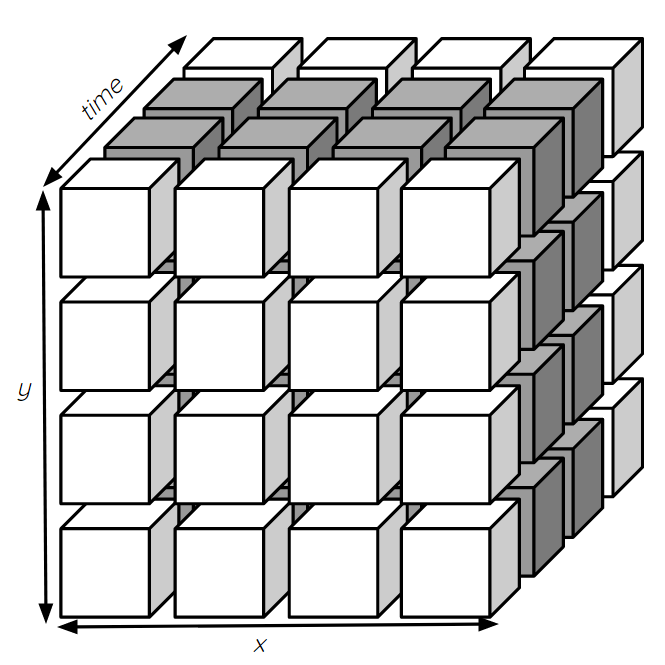
\includegraphics[width=0.3\linewidth]{image/general/atom_time_slicing.PNG}\\
  (a) Region of Interest & (b) Time Slicing
  \end{tabular}
  \caption{Types of Queries: (a) Region of Interest \& (b) Time Slicing}
  \label{fig:typesofQuery}
\end{figure}



\section{Vehicle Blobs Extraction}
\label{subsection:fundamental}

As described in Section~\ref{subsec:scope}, the preliminary task of detecting, tracking and identifying bounding box of vehicles is out of the scope for this work. However, since this task is essential before the semantic extraction task, this section briefly describes the steps taken by \citeA{lim2017} to detect and extract moving objects from video footage. The usage of background subtraction techniques enables the differentiation between static background and moving objects as depicted in Figure~\ref{fig:bgs}.

\begin{figure}[htb!]
  \centering
  \begin{tabular}{cc}
  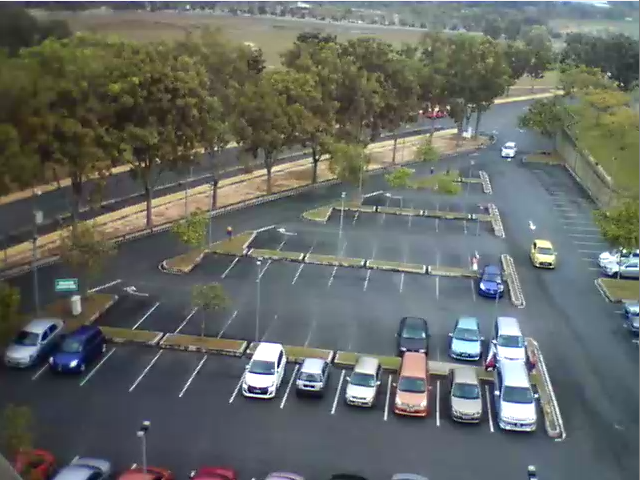
\includegraphics[width=0.4\linewidth]{image/general/bgs1.png} &
  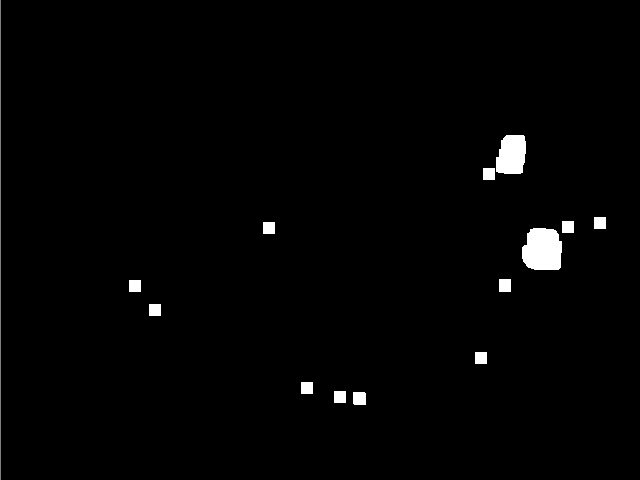
\includegraphics[width=0.4\linewidth]{image/general/bgs2.png}  \\
  (a) 123th frame of a video & (b) Result of background subtraction \\
  \end{tabular}
  \caption{Background Subtraction}
  \label{fig:bgs}
\end{figure}

As the vanilla application of background subtraction (BGS) often results with noisy output, the proposed algorithm used in \cite{lim2017} implemented a combination of adaptive learning and frame differencing method. The BGS method detects and extracts moving objects (henceforth, referred to as foreground blobs).
Several erosion and dilation morphology operations were then performed to further reduce noise and to provide a better representation of foreground blob at the end of the process.
To further improve the accuracy of the extracted blobs, several handcrafted parameters were used to filter out blobs which do not match the dimensions of vehicles.
Furthermore, a deep learning model, was deployed to increase the probability of filtering non-vehicle blobs.


% \begin{comment}
% \begin{figure}[htb!]
%   \centering
% \begin{tabular}{ccc}
%  
\includegraphics[width=0.2\linewidth]{image/general/morph_ori.png} &  
\includegraphics[width=0.2\linewidth]{image/general/morph_erode.png} &
%  
\includegraphics[width=0.2\linewidth]{image/general/morph_dilate.png}\\
% (a) Original Image & (b) Eroded Image & (c) Dilated Image \\
% \end{tabular}
% \caption{Morphology Operations: Erosion \& Dilation}
% \label{fig:morph}
% \end{figure}

% The process is known as \textit{Opening} occurs when the morphology operations are done in the following sequence - 1) Erosion, \& 2) Dilation, noisy data from the background subtraction method can be eliminated as the erosion operation will be able to remove noise while maintaining the important subjects. In contrast, the operation known as \textit{closing} occurs when the dilation step is first performed, followed by the erosion step. This process is useful to fill up the gaps within the foreground objects. These processes are illustrated in Figure~\ref{fig:morph2}

% \begin{figure}[htb!]
%   \centering
% \begin{tabular}{cc}
%  
\includegraphics[width=0.4\linewidth]{image/general/opening.png} &  \includegraphics[width=0.4\linewidth]{image/general/closing.png}  \\
% (a) Opening & (b) Closing \\
% \end{tabular}
% \caption{Morphology Operations: Opening \& Closing}
% \label{fig:morph2}
% \end{figure}


% \cc{do i need to cite these images? \\}
% %https://docs.opencv.org/3.0-beta/doc/py_tutorials/py_imgproc/py_morphological_ops/py_morphological_ops.html
% \end{comment}


The work of ~\citeA{redmon2016you} namely YOLOv2 (You Only Look Once) - a \textbf{real-time} object detection deep learning model was deployed as a complementary module used to classify vehicles and non-vehicle blobs.
As this model focuses on speed, the detection process incurred very little overhead to the overall computational time and cost.
From the foreground blobs, the corresponding bounding boxes were channelled in as inputs for the YOLOv2 network.
%The network will then divide the input into multiple smaller regions and perform prediction of the bounding box along with the class probability.
As the YOLOv2 model is pre-trained with vehicles as one of the many classes, no further retraining was done. The tracking of the blobs only took place if they were identified as vehicles. These bounding boxes were then fed into the proposed semantic extraction framework for further processing.


\section{Semantic Extraction}
\label{section:semanticsExtraction}

The ability to extract vehicle-specific semantics from the scene can present deeper insights valuable for surveillance purposes.
As describe in Section~\ref{subsec:scope}, the two major semantics extracted in the proposed algorithm are (i) \textbf{Vehicle Colour} and (ii) \textbf{Vehicle Trajectory}. Other semantic information such as the time and date which were extracted is briefly discussed as these are simple extraction based on the input file names.
Table~\ref{table:semantics} provides a list of all the extracted semantics in this work.
Emphasis is placed on both the colour and motion semantics extraction process and framework in the following subsections.


\begin{table} \centering
\caption {Types of Extracted Semantics and Methods}
\label{table:semantics}
\begin{tabular}{|l|l|l|}
\hline
\textbf{No.} & \textbf{Semantics Type} & \textbf{Method(s)}                                                                                                          \\ \hline
\textbf{1}   & Date                    & Filename data extraction                                                                                                         \\ \hline
\textbf{2}   & Time                    & Filename data extraction                                                                                                         \\ \hline
\textbf{3}   & Colour                   & \begin{tabular}[c]{@{}l@{}}i) Handcrafted Feature \& Distance Estimation (HSV)\\ ii) Distance Estimation (CIELUV)\end{tabular} \\ \hline
\textbf{4}   & Motion                  & \begin{tabular}[c]{@{}l@{}}i) Handcrafted Feature\\ ii) Collection of Centroid \end{tabular}                                \\ \hline
\textbf{5}   & Object Type             & YOLOv2 (described in~\ref{objecttype})                                                                                                               \\ \hline
\textbf{6}   & Size                    & Bounding box from Background Subtraction                                                                                                      \\ \hline
\end{tabular}

\end{table}

\subsection{Colour Semantic}
\label{subsec:colorsemantics}

In a surveillance setting, colour semantics undoubtedly plays a significant role as it is one of the most common information provided by users when tasked to describe objects from a given event in a particular scene.
Yet, the process of accurately extracting vehicle colour information is extremely challenging, especially in an outdoor setting. Often, the overall scene is affected by various factors such as the ambient illumination during the different hours of the day along with weather conditions.
Examples of several commercially available colour detection products such as the `Nix colour sensor' \cite{nixsensorltd} and `Adafruit RGB sensor' \cite{adafruit} relies on independent calibrated light sources in a controlled environment to extract colour semantics.

While colour terms are commonly derived from the Munsell colour system, there are myriads of available colour terms used in different standards as described in Section~\ref{section:colourterm}.
This creates a new set of challenges as colour terms are often described with differing definitions and tuple values.
Consequently, there is a dire need to address this challenge of extracting and representing colour tuples along with its corresponding colour terms.
Inspirations and ideologies were drawn from the Munsell colour system and applied in this work.
Although the Munsell colour system provided significant research contribution toward colour terms naming, the irregularity along the chroma and value axis does not translate well in a modern colour space as the modern colour spaces are often uniformly distributed along chroma axis (see Figure~\ref{fig:munsell}(b)).

To better represent the colour space, this work utilizes the Hue-Saturation-Value (HSV) colour space for the colour extraction framework.
The use of the HSV colour space is twofold: Firstly, as the HSV colour space closely resembles the Munsell Colour System, it eases the colour representation.
Secondly, the distance between two colours is now intuitive and linear as the values are evenly distributed.
As an added benefit, given that HSV colour space is commonly used, the conversion between the RGB and HSV colour space is seamless and can be easily introduced into the colour semantic framework. Figure~\ref{fig:hsvcylinder} provides a visual representation of the HSV colour space.

\begin{figure}[hbt!]\centering
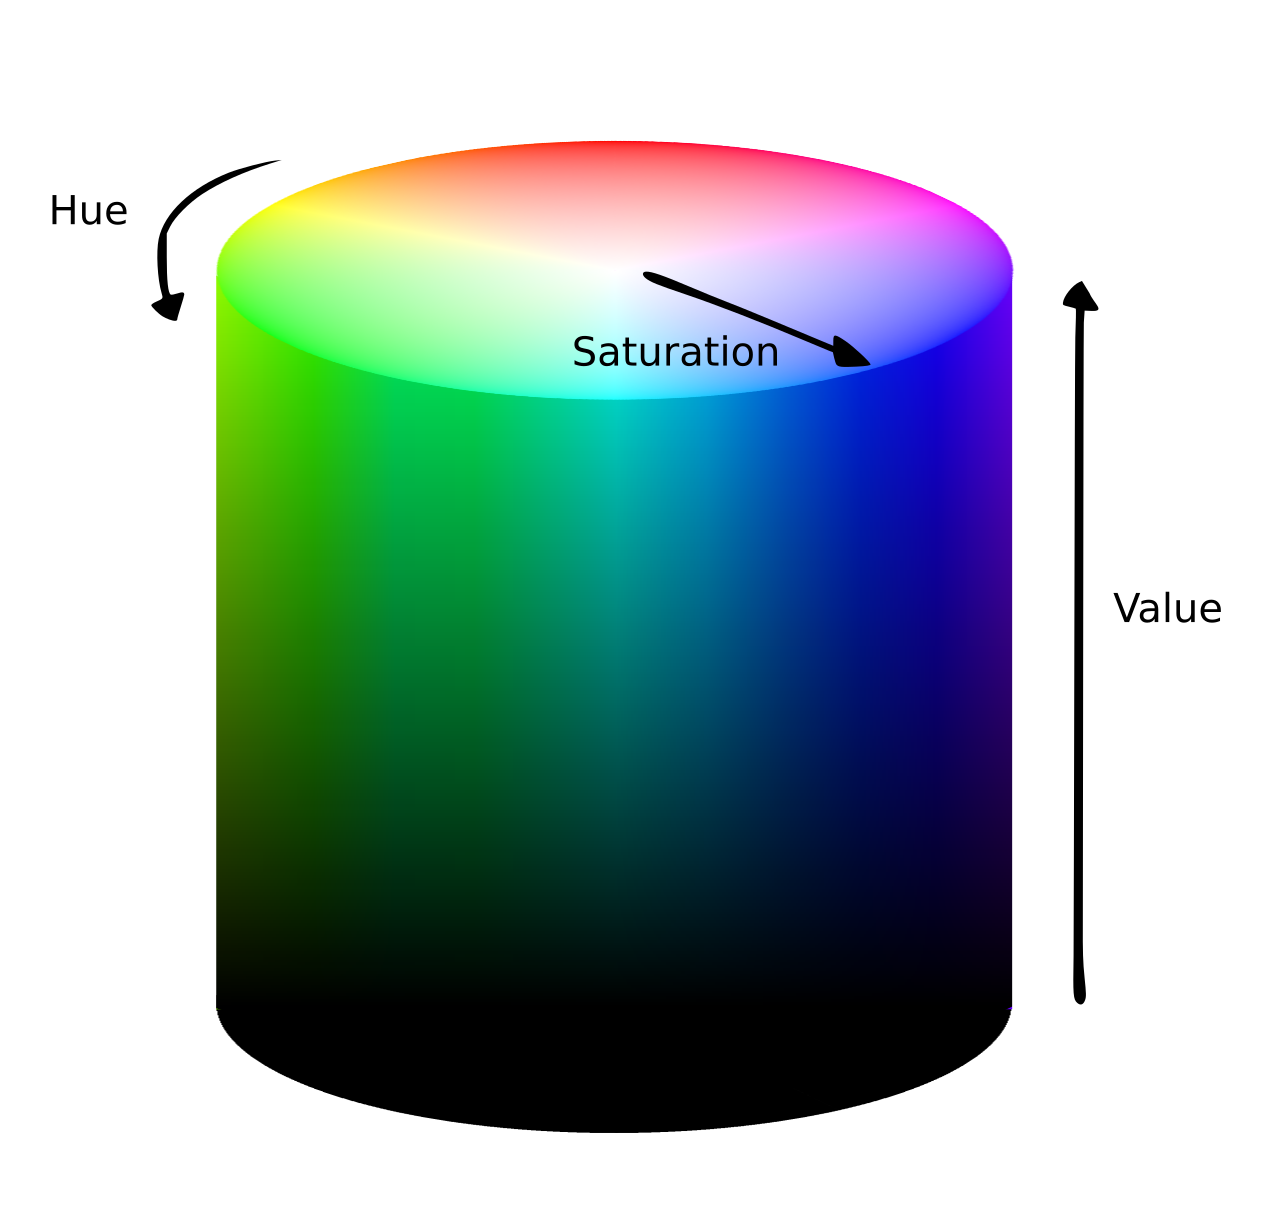
\includegraphics[width=.5\textwidth]{image/general/HSV.png}
\caption{Hue-Saturation-Value (HSV) Cylinder Visualisation}
\label{fig:hsvcylinder}
\end{figure}

Table~\ref{table:allcolourterms} lists several famous web colour dictionary along with the number of colour categories available in each of those colour standards. With so many different colour categories, this ultimately leads to the question of ``\textit{How many colour categories should be extracted for the colour semantic? And why?}''.
To answer the question, the eleven basic colour terms in English proposed by \cite{berlinandkay} was adopted in this work.
\citeA{berlinandkay}'s linguistic approach towards the colour terms assures us that these 11 terms sufficiently describes colours which are often used.
However, the definition of colour terms in itself is insufficient as it invokes another set of challenges - that is, the representation of these colours in \textit{numerical tuples}, such as RGB values which are typically used in computers.
%Bringing it back to the discussion in Section~\ref{section:eyes}, the perception of colour for everyone is relatively different due to the number of cones cells in the retina.
Given that colour perception varies for everyone, compounded with the fact that most monitor screens are not colour calibrated professionally provided an opportunity for Munroe \cite{munroe2010color} to perform an internet crowd-sourcing survey on colour terms and their corresponding numeral representation according to how colours are displayed on typical monitors.

In \citeA{munroe2010color}'s experiment, 222,500 user sessions consisting of 40,000 women and 100,000 men, provided over five million colours their respective terms. With the collected results, Munroe mapped RGB tuples to specific colour terms according to the response frequency.
The mapping of these terms was done by averaging results of several stochastic hill climbing algorithms. At the end of the experiment, 954 colour terms along with its respective RGB tuples were assigned.
Figure~\ref{fig:xkcd} shows the mapping of dominant colour terms over three fully saturated faces of the RGB cube.
By combining the works of \citeA{berlinandkay} and \citeA{munroe2010color}, the eleven basic colour terms can now be mapped to its colour tuples using the information collected. These colour terms and the corresponding HEX values are listed in Table~\ref{table:colorshex}; in this work, these values are treated as \textit{ground truth} values for each colour term.
The details of the techniques used in the semantics extraction process in Phase 1 and Phase 2 will be discussed further in the subsequent sections.

\begin{figure}[!hbt]\centering
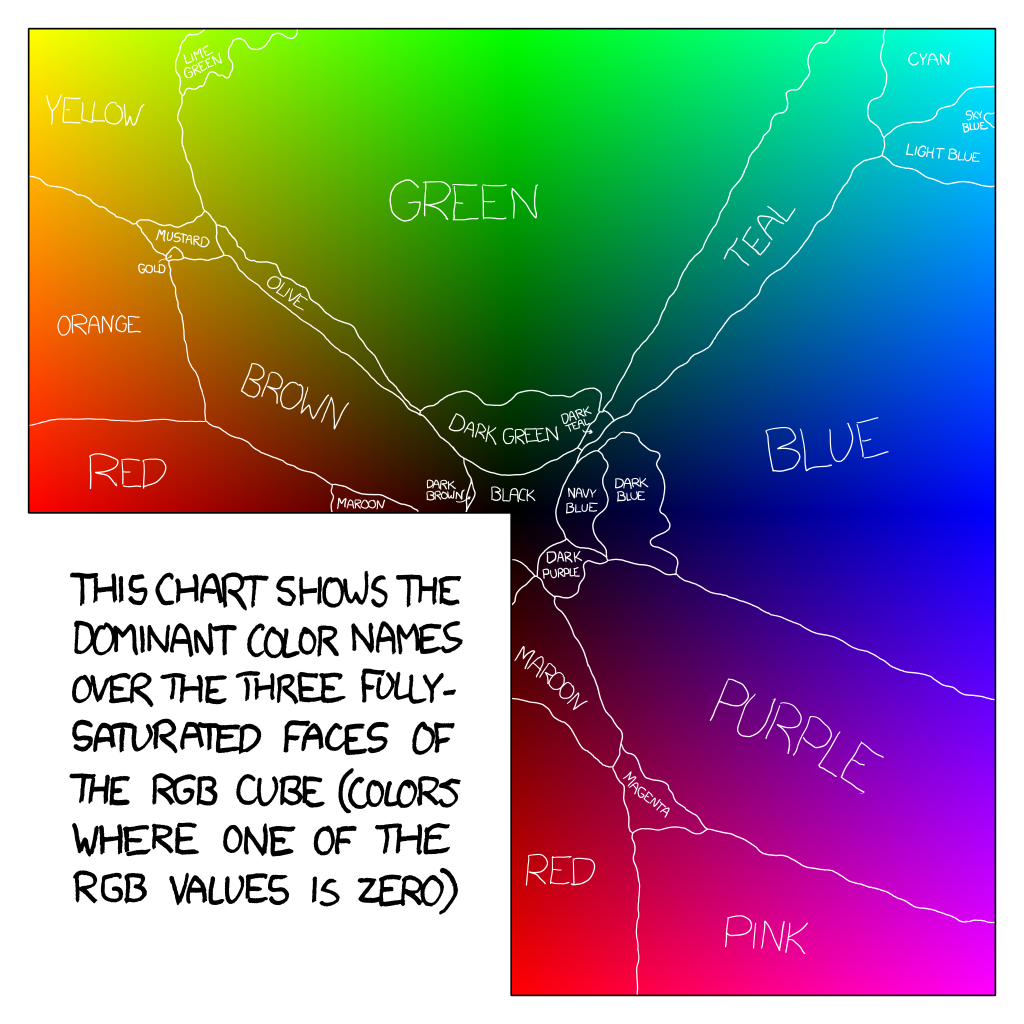
\includegraphics[width=.6\textwidth]{image/general/xkcd.png}
\caption{Dominant Colour Terms over Three Fully Saturated Faces of the RGB Cube}
\label{fig:xkcd}
\end{figure}


% Please add the following required packages to your document preamble:
% \usepackage[table,xcdraw]{xcolor}
% If you use beamer only pass "xcolor=table" option, i.e. \documentclass[xcolor=table]{beamer}
\begin{table}[!ht]\centering
\begin{tabular}{lcccc}
\cline{2-4}
\multicolumn{1}{l|}{}                     & \multicolumn{1}{l|}{\cellcolor[HTML]{000000}} & \multicolumn{1}{l|}{\cellcolor[HTML]{FFFFFF}} & \multicolumn{1}{l|}{\cellcolor[HTML]{929591}} &                                               \\ \cline{1-4}
\multicolumn{1}{|l|}{\textbf{HEX}}        & \multicolumn{1}{c|}{\#000000}                 & \multicolumn{1}{c|}{\#ffffff}                 & \multicolumn{1}{c|}{\#929591}                 &                                               \\ \cline{1-4}
\multicolumn{1}{|l|}{\textbf{Color Term}} & \multicolumn{1}{c|}{Black}                    & \multicolumn{1}{c|}{White}                    & \multicolumn{1}{c|}{Gray}                     &                                               \\ \cline{1-4}
                                          & \multicolumn{1}{l}{}                          & \multicolumn{1}{l}{}                          & \multicolumn{1}{l}{}                          &                                               \\ \cline{2-5}
\multicolumn{1}{l|}{}                     & \multicolumn{1}{l|}{\cellcolor[HTML]{653700}} & \multicolumn{1}{l|}{\cellcolor[HTML]{E50000}} & \multicolumn{1}{l|}{\cellcolor[HTML]{F97306}} & \multicolumn{1}{l|}{\cellcolor[HTML]{FFFF14}} \\ \hline
\multicolumn{1}{|l|}{\textbf{HEX}}        & \multicolumn{1}{c|}{\#653700}                 & \multicolumn{1}{c|}{\#e50000}                 & \multicolumn{1}{c|}{\#f97306}                 & \multicolumn{1}{c|}{\#ffff14}                 \\ \hline
\multicolumn{1}{|l|}{\textbf{Color Term}} & \multicolumn{1}{c|}{Brown}                    & \multicolumn{1}{c|}{Red}                      & \multicolumn{1}{c|}{Orange}                   & \multicolumn{1}{c|}{Yellow}                   \\ \hline
                                          & \multicolumn{1}{l}{}                          & \multicolumn{1}{l}{}                          & \multicolumn{1}{l}{}                          &                                               \\ \cline{2-5}
\multicolumn{1}{l|}{}                     & \multicolumn{1}{l|}{\cellcolor[HTML]{7E1E9C}} & \multicolumn{1}{l|}{\cellcolor[HTML]{15B01A}} & \multicolumn{1}{l|}{\cellcolor[HTML]{0343DF}} & \multicolumn{1}{l|}{\cellcolor[HTML]{FF81C0}} \\ \hline
\multicolumn{1}{|l|}{\textbf{HEX}}        & \multicolumn{1}{c|}{\#7e1e9c}                 & \multicolumn{1}{c|}{\#15b01a}                 & \multicolumn{1}{c|}{\#0343df}                 & \multicolumn{1}{c|}{\#ff81c0}                 \\ \hline
\multicolumn{1}{|l|}{\textbf{Colour Term}}  & \multicolumn{1}{c|}{Purple}                   & \multicolumn{1}{c|}{Green}                    & \multicolumn{1}{c|}{Blue}                     & \multicolumn{1}{c|}{Pink}                     \\ \hline
\end{tabular}
\caption{Colour Terms and the Corresponding HEX value}
\label{table:colorshex}
\end{table}



\subsection{Motion Semantic}

Without a doubt, video data are used for surveillance purposes due to its ability to capture motion information.
Typically, when tasked to describe an event, end-user tends to use a combination of several information such as time of occurrence, description of the objects involved, location and the motion occurred.
Given its importance, this work aims to extract motion semantics from a car park scenario.
In this work, the collective motion performed by a vehicle in the scene is defined as a vehicle's trajectory.
Traditionally, motion information from videos are converted into text-based descriptions using handcrafted methods. For instance, an event such as ``\textit{A yellow vehicle was turning into the intersection between Road Alpha and Road Beta at 3:30 pm when a black vehicle came rushing over and hitting a pedestrian in the process during commotion}'' could be converted into a keyword-based statements such as ``yellow car turn left Road Alpha and Road Beta''.

However, users who are not familiar with the terminology used in the system may find keyword-based statements unintuitive and difficult to decipher.
Furthermore, \cite{bhaumik2016hybrid} claims that the use of textual queries has been proven to be ineffective in video retrieval systems because keywords may not be able to capture the type of semantic content required by an end-user.
While motion information may not be as subjective as the concept of colours, graphical visualization of motion is able to provide clearer info when compared to text-based descriptions.
With that, to provide a more intuitive and natural representation of a given event, this work aims to extract motion information such that it can be represented using graphical form.

Within the scope of a car park scene, the trajectory information from each vehicle is essential as it is used to describe events within the scene.
Hence, it is paramount to ensure motion information from each vehicle is captured and stored accurately.
Given that the types of trajectories performed in a car park varies from user to user, instead of storing these trajectories are a whole, the collected information were quantized and broken down into smaller motion sequence blocks and stored into the database.
As both the proposed motion semantics extraction techniques employ different extraction methods, each phase is discussed separately further down in this chapter.

\subsection{Other Semantic}

In this subsection, the extraction process of the other semantics are briefly described. These extracted semantics includes the date time information, object type as well as object size. As the extractions of these semantics were simple and played little-to-no roles in both the extraction module and retrieval techniques, the extraction processes are described here.

\subsubsection{Date \& Time}

Both date and time data are valuable information in a surveillance setting. In the context of retrieval techniques, these pieces of information are crucial as it can be used to narrow down and filter out irrelevant footage. In this work, the camera was setup to name the recorded files according to the time and date during the dataset collection process. As the filename contains both the time and date information, the date information can be easily obtained via substring extraction. Along with that, when a vehicle is observed in the car park scene, the time information from frame $\mathbb{T}$ can be deduced as follow:
\begin{align}
    \mathbb{T}_{time}  = (\mathbb{VD} \times \frac{\mathbb{T}}{\mathbb{TF}}) + \mathbb{F}_{time}
\end{align}
where $\mathbb{VD}$ corresponds to the video duration of each file (6 minutes) and $\mathbb{TF}$ is the total frames of the current video. The $\mathbb{F}_{time}$ is the time information obtained from the last six digits of filename, excluding the file extension (see Section~\ref{section:dataset_used} for more details). Upon extracting these information, simple formatting is done to ensure these information conform to the typical SQL database requirements.


\subsubsection{Object Type \& Size}
\label{objecttype}
Given that ``vehicles'' are the only object of interest in this work, YOLOv2 was used to assist the validation of the foreground object detected by the BGS method described in Section~\ref{subsection:fundamental}. Objects which were returned under the ``vehicle'' class were tracked are written into the database. As for the object size, the size of the foreground objects' bounding boxes were saved in the database as the object size.


\section{\versionOneExt }
\label{section:semantic_lsh}

\subsection{Overview}
As introduced in Section~\ref{subsec:lsh-intro}, LSH is a hashing function aimed to maximize hash collisions.
As the hashes collide, documents with similar hashes are then grouped and clustered into similar neighbourhoods.
However, LSH techniques were not directly implemented in this work. Instead, the idea and concept of clustering similar semantic classes were drawn.
The extracted semantics are clustered into 11 colour and 9 motion classes, each represented using an SQL table within the database.
This setup allowed quick access to semantic groups while easily representing the classes. Along with that, the proposed method also reduces I/O bottlenecks during the retrieval process as irrelevant tables are ignored.


\begin{figure}[hbt!]\centering
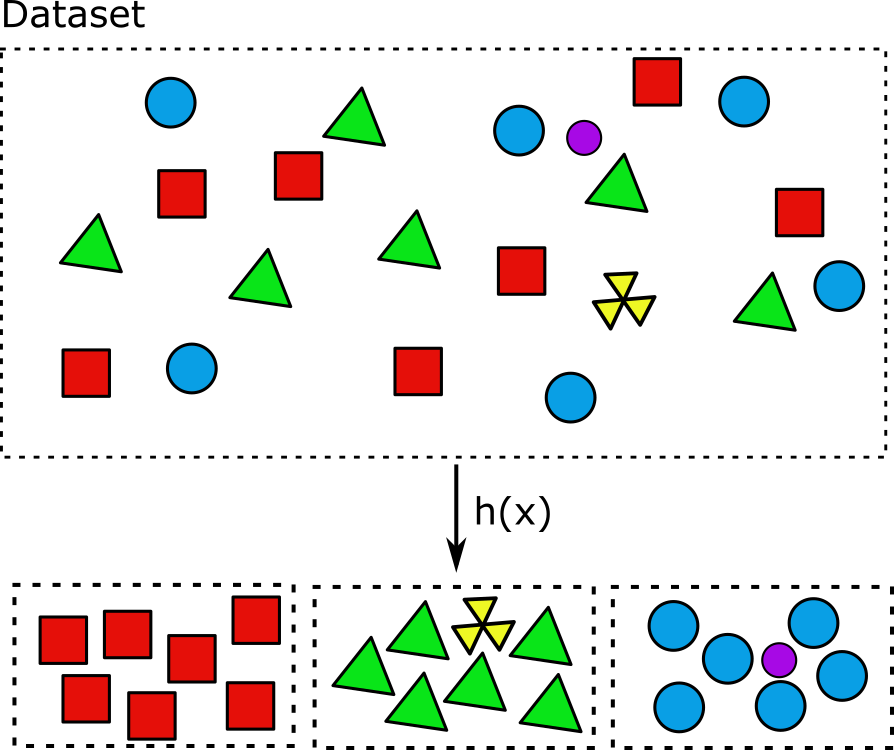
\includegraphics[width=.7\textwidth]{image/new/lsh.png}
\caption{Locality Sensitive Hashing - Documents with Similar Properties Within The Dataset Are Clustered Into Similar Neighbourhood Using LSH Via The Hashing Function, h(x). In This Example, Shapes and Colours are Used to Illustrate Documents With Similar Properties}
\label{fig:lshexample}
\end{figure}

\subsection{Colour Semantic Extraction }
\label{section:versionOneColorExtract}

With the bounding box of the vehicles obtained from the BGS module, the extraction of colour semantics can begin.
However, as the obtained bounding box is larger than the actual vehicle, a cropping function of 30\% towards the centre of the bounding box was introduced to remove unwanted regions.
The cropping function minimizes noise such as surrounding vehicles, roads, and trees from the bounding box, resulting in a closer estimation of the vehicle's footprint.
As the bounding box of each vehicle in this work has very low resolution (approximately around 145$\times$75px), the methods proposed by the other authors in the related work section is neither suitable nor applicable.
%Instead of segmenting portions of the vehicle to extract colour information, the dominant colour of each vehicle is extracted.
To obtain the colour of each vehicle, the first step taken was to distinguish between chromatic and achromatic vehicles.
In this work, the definitions of achromatic colour by Munsell was adopted: Achromatic colours are defined as neutral colours which are characterised by the lack of strong hue or chroma values such as black, white and gray colour.

\begin{figure}[htb!]
  \centering
\begin{tabular}{c}
 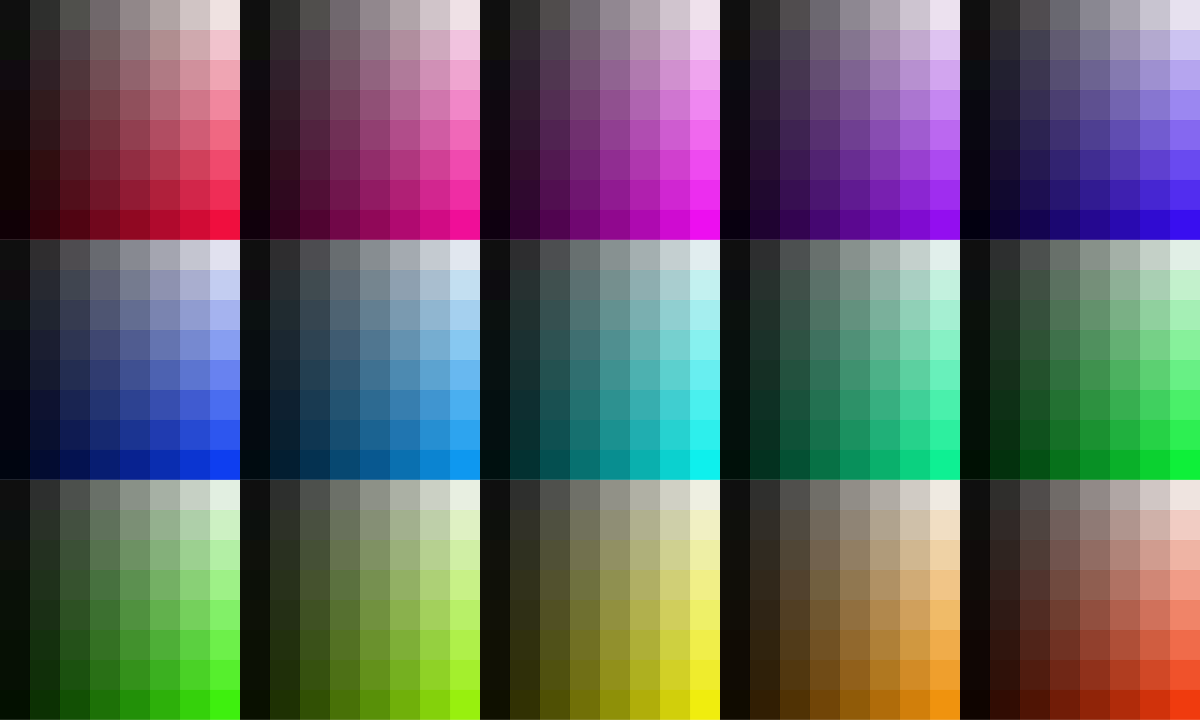
\includegraphics[width=0.7\linewidth]{image/retrievalOne/all.png} \\
\end{tabular}
    \caption{960 Allocated Colour Generated by the 15 Hue, 8 Saturation, \& 8 Value Histogram Bins} \label{fig:hsvAllocated}
\end{figure}

The step to differentiate between chromatic and achromatic vehicles was implemented to overcome the shortcomings of the 960 colour bins proposed for the Colour Term Extraction process.
One of the main drawbacks of the proposed method lies with the number of bins used to represent achromatic colours.
Figure~\ref{fig:hsvAllocated} illustrates the colour bins generated. From the figure, it is clear that there are plenty of bins representing the chromatic tones.
While there are quite many bins representing the black/darker tonnes, only a fraction of bins are used to represent the lighter shades of achromatic colours.
This imbalance, compounded with the achromatic noise captured (ie: road and shadow) during the colour extraction process made it extremely difficult for vehicles to be matched with ``White'' or ``Gray'' colour terms. Hence, this step was introduced as a measure to counterbalance the weakness of the proposed method.
The details on how these colour bins were allocated is discussed later in the chapter.

This process of differentiating chromatic against achromatic vehicles starts by comparing the cropped image, $I_{crop}$, against a grayscale version, $I_{gray}$.
The conversion from RGB to grayscale is performed using $I_{gray} = 0.299 \cdot I_{crop}[R]+0.587 \cdot I_{crop}[G]+0.114 \cdot I_{crop}[B]$.
As grayscale images and RGB images do not have the same number of channels, the grayscale image is converted back to into a 3 channel image.
Next, the absolute difference between these images are obtained using: $I_{Abs_{diff}} = \mid I_{crop} - I_{gray(RGB)} \mid$.
However, the difference produced tend to be rather low.
Hence, the next step is to subject the obtained $I_{Abs_{diff}}$ result to a thresholding process for all 3 channels in the RGB colour space to produce $I_{threshold}(RGB)$.
The step effectively amplifies the difference between the original image and the grayscale image. Pixels, $Pv_{(x,y)}$, with values above the threshold value of 35 were set to the maximum value of 255.
Finally, the output %of $I_{threshold}(RGB)$
is converted back to the grayscale colour space to generate $I_{threshold}(gray)$. The hint of significant values at this stage indicates a substantial presence of chromatic hues for this particular vehicle.

\begin{align*}
\label{eq:threshabsolutediff}
I_{threshold}(x,y)(RGB) = \alpha \cdot (255) \\
\text{where, }
\alpha =
\begin{cases}
1, & Pv_{(x,y)} \geq 35\\
0, & otherwise
\end{cases}
\end{align*}



\begin{comment}
\begin{align}
\label{eq:achromaticSteps}
I_{ori_{i,j}} = \{R_{i,j},G_{i,j},B_{i,j}\} \\
I_{grayscale}, Y_{i,j} = 0.299 \cdot I_{ori}R_{(x_i,y_j)}+0.587 \cdot I_{ori}G_{(x_i,y_j)}+0.114 \cdot I_{ori}B_{(x_i,y_j)}\\
I_{grayscale(RGB_{i,j})} = \begin{cases}R = Y_{i,j}\\G = Y_{i,j} \\ B = Y_{i,j} \end{cases}\\
Abs_{diff}(R,G,B) = \mid I_{ori} - I_{grayscale(BGR)} \mid \\
Threshold_{Abs_{diff}}, T_{Abs_{diff}} =
\begin{cases}R = \begin{cases}Abs_{diff}R\geq 35, & R =255\\ otherwise, & R =0
\end{cases} \\
G = \begin{cases}Abs_{diff}G\geq 35, & G =255\\ otherwise, & G =0
\end{cases} \\
B = \begin{cases}Abs_{diff}B\geq 35, & B =255\\ otherwise, & B =0
\end{cases}
\end{cases}\\
Threshold_{Abs_{diff(grayscale)}} = \\
0.299 \cdot T_{Abs_{diff}}R_{(x_i,y_j)}+0.587 \cdot T_{Abs_{diff}}G_{(x_i,y_j)}+0.114 \cdot T_{Abs_{diff}}B_{(x_i,y_j)}
\end{align}
\end{comment}

With the interest of differentiating between chromatic and achromatic vehicles, the ratio of non-zero pixel value over the total pixels within the bounding box is obtained.
A threshold pivot value, $T_{pivot}$, is assigned to determine if the vehicle belongs to chromatic or achromatic class.
The threshold value is empirically set at 18\% to where vehicles blobs that exceed this value is assumed to contain the presence of strong chromatic hues.
The entire process from the cropped image to the deduction of chromatic class can be illustrated using Figure~\ref{fig:achromatic_thresh}. This handcrafted algorithm allows the deduction of strong chromatic hues and estimates if a particular vehicle blob belongs to a chromatic or achromatic subset.

\begin{figure}[htb!]
  \centering
\begin{tabular}{c}
 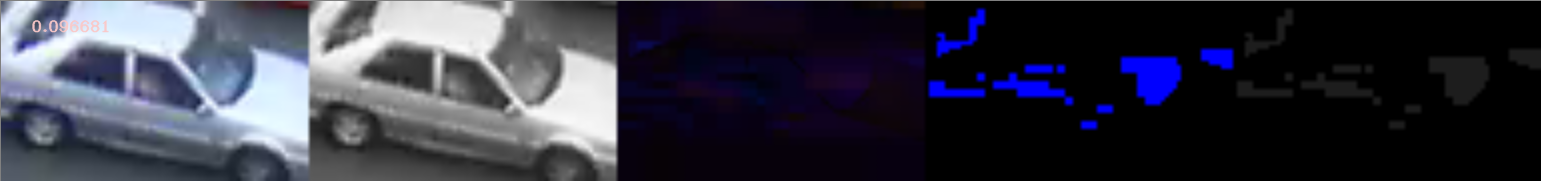
\includegraphics[width=0.9\linewidth]{image/general/achromatic_threshold5.PNG} \\
 (a) Achromatic vehicle (Gray/White) \\
 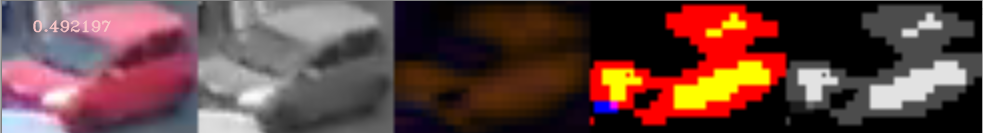
\includegraphics[width=0.9\linewidth]{image/general/achromatic_threshold_color2.PNG}\\
(b) Chromatic vehicle (Red)
\end{tabular}
\caption{(From left) Original image, $I_{crop}$; Grayscale image, $I_{gray}$; Absolute difference, $I_{Abs_{diff}}$; Binary threshold absolute difference, $I_{threshold}(RGB)$; Threshold difference in grayscale, $I_{threshold}(gray)$} \label{fig:achromatic_thresh}
\end{figure}

\paragraph{Achromatic and chromatic colour processing.} Upon determining vehicle belonging to the achromatic class, the cropped images are then subjected to both the black and white colour filters individually. These simple filters were designed using binary thresholds values empirically set at an intensity level of 50 and 170 respectively.
Using a similar fashion, the ratio of non-zero pixels upon filtering is computed. The obtained ratio is then used to determine if the vehicle belongs to black, white or gray colour groups. Figure~\ref{fig:blackwhite_filter} illustrates the response map of a white vehicle towards both the black and white filters.
The colour terms are then assigned to the vehicles based on the results.

\begin{figure}[htb!]
  \centering
\begin{tabular}{ccc}
 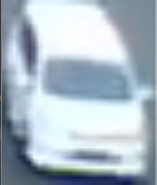
\includegraphics[width=0.22\linewidth]{image/retrievalOne/whitefilter1.png}   &
 
\includegraphics[width=0.22\linewidth]{image/retrievalOne/whitefilter2.png}   &
 
\includegraphics[width=0.22\linewidth]{image/retrievalOne/whitefilter3.png}   \\
(a) Target Vehicle (White) &
(b) Black Filter Response &
(c) White Filter Response \\
\end{tabular}
\caption{Black \& While Filter Response of a White Vehicle} \label{fig:blackwhite_filter}
\end{figure}


 \begin{algorithm}[!ht]
  \caption{Achromatic Colour Term Extraction}
  \label{algo:achromatic}
  \begin{algorithmic}[1]

  \IF{Percentage of White $>$ 25\%  \\
  \hspace{1em} \&\& Percentage of Black $<$ 25\%}
    \STATE Colour Term = White
  \ELSIF {Percentage of Black $>$ 25\%  \\
  \hspace{1em} \&\& Percentage of White $<$ 25\%}
      \STATE Colour Term = Black
  \ELSE
      \STATE Colour Term = Gray
  \ENDIF

  \end{algorithmic}
\end{algorithm}


 \begin{algorithm}[!ht]
  \caption{Colour Term Extraction}
  \label{algo:colorExtract}
  \begin{algorithmic}[1]
    \FOR{Each blob in image}
        \STATE Shrink bounding box \& crop image
        \STATE Create a copy of the cropped image in grayscale
        \STATE Compute the absolute difference between cropped image \& grayscale image
        \STATE Perform threshold on absolute difference to amplify the difference
        \STATE Convert results into grayscale \& calculate no. of non-zero pixels
            \IF{Ratio of non-zero pixels $>$ $T_{pivot}$}
                \STATE // Chromatic Vehicle
                \STATE Calculate 3D HSV histogram
                \STATE Locate maximum bin location of each channel
                \STATE Map the highest bin from each channel to Colour Term
            \ELSE
                \STATE // Achromatic Vehicle
                \STATE Perform black \& white filter
                \STATE Obtain ratio of non-zero pixels from both filters
                \STATE CALL: Achromatic Colour Term Extraction
            \ENDIF

    \ENDFOR
    \STATE Obtain average dominant colour \& return Colour Term
  \end{algorithmic}
\end{algorithm}

Contrary to the achromatic vehicle class, the chromatic class utilizes a different method of determining colour terms.
%As previously mentioned, this work chose to primarily work on the HSV colour space, especially for the chromatic colour extraction process.
First, the cropped RGB image is converted to the HSV colour space. Then, a 3-Dimensional histogram of the cropped image is generated.
As colours belong to a spectrum, the HSV histogram is quantized into 15 Hue, 8 Saturation and 8 Value bins.
While a finer-grained histogram might be able to produce higher accuracy when representing the vehicle's colour, the results may not be ideal as the generated output would spread across a larger segment.
The $15-8-8$ configuration is inspired by the works of \cite{kim2008deciding}. Their experiments show that the $8-4-4$ configuration showed the best results.
The chosen configuration doubles up the proposed number of bins used in the histogram, this approach of doubling the bins across all 3 channels would produce a sufficiently accurate representation of the vehicle colour.
The decision to use 15 bins instead of 16 bins for the Hue channel is because hues are represented using 360$^{\circ}$. To divide 360$^{\circ}$ evenly, 15 bins were chosen.


% Please add the following required packages to your document preamble:
% \usepackage[table,xcdraw]{xcolor}
% If you use beamer only pass "xcolor=table" option, i.e. \documentclass[xcolor=table]{beamer}
\begin{table}[!ht]\centering
\resizebox{\textwidth}{!}{
\begin{tabular}{c|c|c|c|c|c|c|c|c|c|c|c|}
\cline{2-12}
\multicolumn{1}{l|}{}                        & \multicolumn{11}{c|}{\textbf{Similarity(\%) Based on $D_{Euclidean}$ in HSV Colour Space}}                                                                                                                                                                                       \\ \hline
\multicolumn{1}{|c|}{\textbf{Bin/Colour}} & \textbf{Black} & \textbf{Blue} & \textbf{Brown} & \textbf{Gray}                          & \textbf{Green}                         & \textbf{Orange} & \textbf{Pink}                          & \textbf{Purple}                        & \textbf{Red} & \textbf{White} & \textbf{Yellow} \\ \hline
\multicolumn{1}{|c|}{
\begin{tabular}{c}  \\

\includegraphics[width=0.1\linewidth]{image/HSVcolorspace/img_0_4_7.jpg} \\
\textbf{0, 4, 7}
\end{tabular}     }

& 30.46          & 67.06         & 55.74          & 57.51                                  & 70.94                                  & 73.76           & \cellcolor[HTML]{9AFF99}\textbf{92.18} & 71.95                                  & 72.25        & 64.00          & 76.33           \\ \hline

\multicolumn{1}{|c|}{
\begin{tabular}{c}  \\

\includegraphics[width=0.1\linewidth]{image/HSVcolorspace/img_2_4_3.jpg} \\
\textbf{2, 4, 3}
\end{tabular}     }


& 54.07          & 60.33         & 70.03          & 59.16                                  & 66.14                                  & 55.81           & 64.00                                  & \cellcolor[HTML]{9AFF99}\textbf{81.03} & 59.25        & 49.04          & 55.33           \\ \hline

\multicolumn{1}{|c|}{
\begin{tabular}{c}  \\

\includegraphics[width=0.1\linewidth]{image/HSVcolorspace/img_3_7_4.jpg} \\
\textbf{3, 7, 4}
\end{tabular}     }

& 29.70          & 73.77         & 86.97          & 42.04                                  & \cellcolor[HTML]{9AFF99}\textbf{90.03} & 72.85           & 58.01                                  & 78.43                                  & 76.15        & 33.49          & 72.24           \\ \hline
\multicolumn{1}{|c|}{
\begin{tabular}{c}  \\

\includegraphics[width=0.1\linewidth]{image/HSVcolorspace/img_6_2_6.jpg} \\
\textbf{6, 2, 6}
\end{tabular}     }


& 41.35          & 56.33         & 46.77          & \cellcolor[HTML]{9AFF99}\textbf{75.87} & 62.87                                  & 53.88           & 72.91                                  & 62.49                                  & 52.12        & 69.89          & 58.04           \\ \hline



% ----- remove these?

\multicolumn{1}{|c|}{
\begin{tabular}{c}  \\

\includegraphics[width=0.1\linewidth]{image/HSVcolorspace/img_11_0_0.jpg} \\
\textbf{11, 0, 0}
\end{tabular}     } &

\cellcolor[HTML]{9AFF99}\textbf{88.15} &    21.74 &    35.36 &    60.73 &    31.88 &    17.02 &    34.30 &    41.36 &    19.80 &    39.59 &    17.52
\\ \hline

\multicolumn{1}{|c|}{
\begin{tabular}{c}  \\

\includegraphics[width=0.1\linewidth]{image/HSVcolorspace/img_11_0_1.jpg} \\
\textbf{11, 0, 1}
\end{tabular}     }  &
\cellcolor[HTML]{9AFF99}\textbf{83.66} &    26.71 &    37.51 &    67.13 &    36.19 &    22.35 &    41.39 &    45.70 &    24.80 &    47.38 &    23.04
\\ \hline

\multicolumn{1}{|c|}{
\begin{tabular}{c}  \\

\includegraphics[width=0.1\linewidth]{image/HSVcolorspace/img_11_0_2.jpg} \\
\textbf{11, 0, 2}
\end{tabular}     }  &
\cellcolor[HTML]{9AFF99}\textbf{77.20} &    31.13 &    38.69 &    72.71 &    39.75 &    27.21 &    48.22 &    49.15 &    29.27 &    55.12 &    28.11
\\ \hline

\multicolumn{1}{|c|}{
\begin{tabular}{c}  \\

\includegraphics[width=0.1\linewidth]{image/HSVcolorspace/img_11_0_3.jpg} \\
\textbf{11, 0, 3}
\end{tabular}     }  &
70.02 &    34.87 &    38.85 &    \cellcolor[HTML]{9AFF99}\textbf{76.86} &    42.43 &    31.48 &    54.68 &    51.54 &    33.08 &    62.76 &    32.61
\\ \hline

\multicolumn{1}{|c|}{
\begin{tabular}{c}  \\

\includegraphics[width=0.1\linewidth]{image/HSVcolorspace/img_11_0_4.jpg} \\
\textbf{11, 0, 4}
\end{tabular}     }  &
62.53 &    37.82 &    37.98 &    \cellcolor[HTML]{9AFF99}\textbf{78.73} &    44.10 &    35.06 &    60.60 &    52.69 &    36.13 &    70.25 &    36.44
\\ \hline

\multicolumn{1}{|c|}{
\begin{tabular}{c}  \\

\includegraphics[width=0.1\linewidth]{image/HSVcolorspace/img_11_0_5.jpg} \\
\textbf{11, 0, 5}
\end{tabular}     }  &
54.88 &    39.85 &    36.13 &    \cellcolor[HTML]{9AFF99}\textbf{77.73} &    44.67 &    37.83 &    65.69 &    52.53 &    38.30 &    77.42 &    39.47
\\ \hline

\multicolumn{1}{|c|}{
\begin{tabular}{c}  \\

\includegraphics[width=0.1\linewidth]{image/HSVcolorspace/img_11_0_6.jpg} \\
\textbf{11, 0, 6}
\end{tabular}     }  &
47.14 &    40.88 &    33.38 &    74.20 &    44.10 &    39.67 &    69.54 &    51.05 &    39.50 &    \cellcolor[HTML]{9AFF99}\textbf{83.84} &    41.56
\\ \hline

\multicolumn{1}{|c|}{
\begin{tabular}{c}  \\

\includegraphics[width=0.1\linewidth]{image/HSVcolorspace/img_11_0_7.jpg} \\
\textbf{11, 0, 7}
\end{tabular}     }  &
39.35 &    40.84 &    29.83 &    68.98 &    42.43 &    40.49 &    71.62 &    48.38 &    39.665 &    \cellcolor[HTML]{9AFF99}\textbf{88.23} &    42.61
\\ \hline


% ----- remove these?

\end{tabular}}
\caption{Samples of Similarity Score(\%) based on Euclidean Distance in HSV Colour Space, Highlighted in Green is the Highest Scoring Colour Term}
\label{tab:hsvExample}
\end{table}


This $15-8-8$ configuration ends up with a total of 960 histogram bins (See Figure~\ref{fig:hsvAllocated}).
Each of these bins is then assigned a \textit{single colour term} based on the closest Euclidean distance between the bin's colour and the highest scoring ground truth colour term using the HSV colour space.
Instead of storing the histogram details of each vehicle, only the histogram bin with the highest number of hits is utilized.
Essentially, these bins would represent the most dominant colour of the vehicle.% at a particular video frame, $\alpha_T$.
%Using the colour terms obtained for that particular histogram bin, the vehicle colour at $V_T$ is stored in the database.

As the vehicles' bounding boxes were obtained and tracked when they were moving, the vehicle colour may vary depending on surrounding, ambient lighting, and shadows.
Hence, the dominant colour of a vehicle at frame $\alpha_T$, is obtained and stored in the database. This setup allows vehicles to be classified with a variety of colours at different time frame.
Algorithm~\ref{algo:colorExtract} summarises the strategy used for colour semantic extraction process for the \versionOneExt,
while the examples in Table~\ref{tab:hsvExample} shows samples of bins and their corresponding similarity score.


\subsection{Motion Semantic Extraction}
\label{subsec:motions9binextract}

To extract motion information from the vehicles, the bounding box obtained from the BGS method is used.
Using the bounding box, the location of each vehicle is obtained using its respective centroids (Equation~\ref{eq:centroid}).
The motion information is then extracted using a naive inference of the motion displacement obtained from the X and Y-axis.
Furthermore, the centroid obtained from the vehicle at each frame ($P_N$) is stored in a list, \H{L}.
As two subsequent frames are likely to have minimal differences, the algorithm was set to wait until the \H{L} list has at least 10 records (approximating the width of 1 $\alpha_T$, or 10 frames) of the previous position before extracting the motion information.
Algorithm~\ref{algo:motion} provides details of this semantic extraction process in pseudo-code.

During this phase, the motion of a vehicle is quantized into 8 directional bins using four cardinal directional, four intermediate directional bins and another bin which denotes minuscule or negligible motions.
These quantized directions can then be categorised into one of the 9 motions using: UP, DOWN, LEFT, RIGHT, LEFT-UP, LEFT-DOWN, RIGHT-UP, RIGHT-DOWN, MOTIONLESS.
Figure~\ref{fig:cardinalbins} illustrates the motion bins and the corresponding directions.
Each of these directions are determined using handcrafted parameters, the displacement values ($X_{displacement}$ \& $Y_{displacement}$) are empirically selected set at 5 pixels respectively.
In the scenario where the difference between the current position of the centroid and the position 10 frames ago is larger than either $X_{displacement}$ or $Y_{displacement}$, the motion of the vehicle will then be updated and save into the database accordingly for each frame.

\begin{figure}[H]\centering
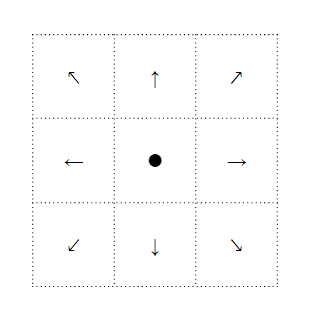
\includegraphics[width=.5\textwidth]{image/new/motion.PNG}
\caption{Directional bins setup}
\label{fig:cardinalbins}
\end{figure}


 \begin{algorithm}[H]
    \caption{Motion Semantic Extraction}
    \label{algo:motion}
    \begin{algorithmic}[1]
        \FOR{Each blob}
        \STATE Save current centroid position ($P_N$) in $List_{motion}$, \H{L}
        \IF{\H{L}.length > 10}
        \STATE Calculate $Difference_x$ and $Difference_y$ using:
        \STATE $Difference_{centroid} = P_N -P_{(N-10)}$
        \IF {Absolute ($Difference_{x}$) > $X_{displacement}$ }
        \IF {$Difference_{x}$ > 0 }
        \STATE Set \textit{Direction(X)} to "LEFT"
        \ELSE
        \STATE Set \textit{Direction(X)} to "RIGHT"
        \ENDIF
        \ENDIF
        \IF {Absolute ($Difference_{y}$) > $Y_{displacement}$ }
        \IF {$Difference_{y}$ > 0 }
        \STATE Set \textit{Direction(Y)} to "UP"
        \ELSE
        \STATE Set \textit{Direction(Y)} to "DOWN"
        \ENDIF
        \ENDIF

        \IF {\textit{Direction(Y)} != NULL AND \textit{Direction(X)} != NULL }
        \STATE Set blob's motion = \textit{Direction(X)} + \textit{Direction(Y)}
        \ELSE
        \IF {\textit{Direction(X)} != NULL }
        \STATE Set blob's motion = \textit{Direction(X) }
        \ELSIF  {\textit{Direction(Y)} != NULL }
        \STATE Set blob's motion = \textit{Direction(Y)}
        \ELSE
        \STATE Set blob's motion = "Motionless"
        \ENDIF
        \ENDIF
        \ENDIF
        \STATE Save blob's current motion into database
        \ENDFOR
    \end{algorithmic}
\end{algorithm}



\section{\versionTwoExt }
\label{section:semantic_chamfer}

\subsection{Overview}

Upon experimenting with the methods proposed in Phase 1, one of the main shortcoming identified was that the extracted semantics was too handcrafted.
As a result, the input of the retrieval technique had to be meticulously and precisely selected to achieve optimum results (see Section~\ref{section:versionOne}).
Although the results could potentially be improved with further careful tweaking of the various parameters, the experimental process for what works best would be extremely tedious.
Furthermore, the selected parameters would not necessarily be extendable to other works working on a different set of input data.

Along with that, there were several other key issues identified that could be improved upon.
The experimental results show that the process of determining between achromatic and chromatic vehicles were particularly problematic.
The experimental dataset highlighted positive bias towards achromatic vehicles as there were a lot more achromatic vehicle as compared to chromatic vehicle.
Given the bias scale, it is a trivial task to manipulate the overall retrieval results by adjusting the parameters to favour the achromatic scale.
Hence, the aim of Phase 2: \versionTwoExt is to implement alternative solutions with better performance when compared with Phase 1: \versionOneExt. In the next subsections, the colour semantic extraction and motion semantic extraction is discussed in detail.


\subsection{Colour Semantic Extraction}
\label{section:versiontwoColor}
As previously discussed in the section~\ref{subsec:colorsemantics}, while the fundamental idea of discerning colours terms is relatively simple for humans, machines have a hard time grasping the concept of colours. To extract colour semantics, the framework from Phase 1 was inherited and modified.
First, the dominant colour from each frame is extracted using the 3D HSV histogram bin observed with the highest number of hits. Next, the dominant colour from each frame is concatenated into an image. At the end of a vehicle's tracked life cycle, the concatenated dominant colours are averaged out to obtain the Average Dominant Colour (ADC). The example in Figure~\ref{fig:ADC} illustrates the process taken by this method while the pseudo-code of the ADC method is described in Algorithm~\ref{algo:ADC}.

\begin{figure}[hbt!]\centering
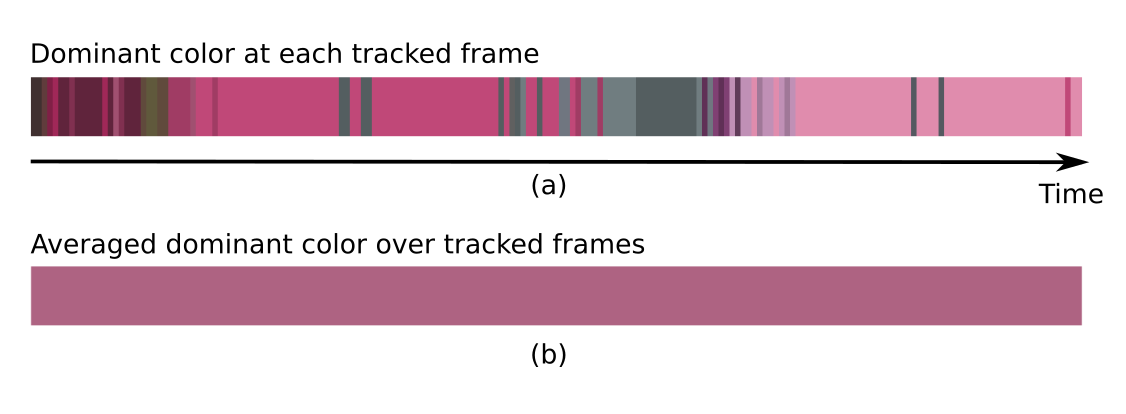
\includegraphics[width=.9\textwidth]{image/general/ADC.png}
\caption{(a) Dominant Colour of the Vehicle at Each Frame; (b) Average Dominant Colour (ADC)}
\label{fig:ADC}
\end{figure}

\begin{algorithm}[H]
  \caption{Average Dominant colour \& Similarity Score Determination}
  \label{algo:ADC}
  \begin{algorithmic}[1]
    \FOR{Each tracked vehicle in the current frame}
        \STATE Shrink bounding box (crop image)
        \STATE Calculate 3D HSV histogram
        \STATE Locate maximum bin location of each channel from histogram
        \STATE Concatenate resulting dominant colours from each frame
        \STATE Obtain the Average Dominant colour (ADC)
        \STATE Measure the difference between ground truth value (Table~\ref{table:colorshex}) and ADC
        \STATE Obtain Similarity Score of colour tuple against colour terms
    \ENDFOR
  \end{algorithmic}
\end{algorithm}

To reduce the number of parameters and steer clear of handcrafted features such as the one introduced in Phase 1, the usage of similarity scores were adopted in Phase 2.
Instead of assigning a single colour term for each of the 960 histogram bins, the similarity score of the ADC against \textbf{all} eleven ground truth colours is calculated and saved into the database. The metrics used to measure the similarity scores between the colours is adopted from the work of Riemersma\cite{riemersma}. The author proposed a low-cost estimation of the differences for colours in the LUV linear colour space using RGB values. As the Average Dominant colour was obtained in the HSV colour space, a quick conversion from HSV to RGB colour space was done using Equation~\ref{eq:RGBHSVconversion1} to~\ref{eq:RGBHSVconversion3}.



%% ---- RGBHSVconversion metric ------------------------------------------------
\begin{equation}
\label{eq:RGBHSVconversion1}
V = \max(R,G,B)
\end{equation}

\begin{equation}
\label{eq:RGBHSVconversion2}
S = \begin{cases}\frac{V - \min(R,G,B)}{V} & , V \neq 0\\
0 & , otherwise \end{cases} \\
\end{equation}

\begin{equation}
\label{eq:RGBHSVconversion3}
H = \begin{cases}
\hspace{2.8em} \frac{60(G-B)}{V-\min(R,G,B)} & ,V = R\\
120 + \frac{60(B-R)}{V-\min(R,G,B)} & ,V = G\\
240 + \frac{60(R-G)}{V-\min(R,G,B)} & ,V = B
\end{cases}
\end{equation}

\centerline{\\$\textit{if } \hspace{.8em}H< 0 \hspace{.8em}\textit{ then } \hspace{.8em}H = H+360.$}


%% ---- RGBHSVconversion metric ------------------------------------------------


According to Riemersma, the benefit of this metrics is that it is a far more stable algorithm where, as quoted, ``it does not have a range of colours where it suddenly gives far from optimal results''. First, the mean of both the Average Dominant Colour (ADC) and Ground Truth colour (GTC)'s red channel is obtained. Then, this is followed by obtaining the difference, $\Delta$, of all three R, G, and B channels.
In Equation~\ref{eq:DiffColorLUV}, the mean of the red channel ($\mean{r}$) is used as a weight for both $\Delta{R}$ and $\Delta{B}$. The details of these equations is described in Equation~\ref{eq:RedMeanRGBDiff} and~\ref{eq:DiffColorLUV} respectively. Table~\ref{tab:luvExample} uses the same example colours as used in Table~\ref{tab:hsvExample}, however, the similarity score of the colours are calculated using the metric suggested in Equation~\ref{eq:DiffColorLUV} instead of the Euclidean Distance measured in HSV colour space.

%% ---- First metric ------------------------------------------------
\begin{equation}
\begin{split}
\label{eq:RedMeanRGBDiff}
\mean{r} = \frac{C_{1R} + C_{2R}}{2}
\end{split}
% \end{equation}
\quad\quad\quad ; \quad\quad\quad
% \begin{equation}
 \begin{split}
\Delta R = C_{1R} - C_{2R}\\
\Delta G = C_{1G} - C_{2G}\\
\Delta B = C_{1B} - C_{2B}
 \end{split}
\end{equation}

\begin{equation}
\label{eq:DiffColorLUV}
\Delta Colour_{LUV} = \sqrt{(2 + \frac{\mean{r}}{256}) \times \Delta R^{2} + 4 \times \Delta G^{2} + (2 + \frac{255 - \mean{r}}{256}) \times \Delta B^{2} }
\end{equation}




%% ---- First metric ------------------------------------------------



% Please add the following required packages to your document preamble:
% \usepackage[table,xcdraw]{xcolor}
% If you use beamer only pass "xcolor=table" option, i.e. \documentclass[xcolor=table]{beamer}
\begin{table}[!hbt]\centering
\resizebox{\textwidth}{!}{
\begin{tabular}{c|c|c|c|c|c|c|c|c|c|c|c|}
\cline{2-12}
\multicolumn{1}{l|}{}                        & \multicolumn{11}{c|}{\textbf{Similarity(\%) Based on Riemersma's low cost LUV estimation metrics}}                                                                                                                                                                                       \\ \hline
\multicolumn{1}{|c|}{\textbf{Bin/Colour}} & \textbf{Black} & \textbf{Blue} & \textbf{Brown} & \textbf{Gray}                          & \textbf{Green}                         & \textbf{Orange} & \textbf{Pink}                          & \textbf{Purple}                        & \textbf{Red} & \textbf{White} & \textbf{Yellow} \\ \hline
\multicolumn{1}{|c|}{
\begin{tabular}{c}  \\

\includegraphics[width=0.1\linewidth]{image/HSVcolorspace/img_0_4_7.jpg} \\
\textbf{0, 4, 7}
\end{tabular}     }

&
0.00 &     0.91 &     28.25 &     61.27 &     14.33 &     67.17 &     \cellcolor[HTML]{9AFF99}\textbf{70.97} &     34.74 &     31.11 &     25.76 &     37.78

\\ \hline

\multicolumn{1}{|c|}{
\begin{tabular}{c}  \\

\includegraphics[width=0.1\linewidth]{image/HSVcolorspace/img_2_4_3.jpg} \\
\textbf{2, 4, 3}
\end{tabular}     }


&
34.11 &    22.06 &    \cellcolor[HTML]{9AFF99}\textbf{68.39} &    59.91 &    56.72 &    46.89 &    27.22 &    46.24 &    31.23 &    0.00 &    15.51
\\ \hline

\multicolumn{1}{|c|}{
\begin{tabular}{c}  \\

\includegraphics[width=0.1\linewidth]{image/HSVcolorspace/img_3_7_4.jpg} \\
\textbf{3, 7, 4}
\end{tabular}     }

&
28.13 &    6.53 &    59.41 &    46.70&    \cellcolor[HTML]{9AFF99}\textbf{71.77} &    39.83 &    11.63 &    24.39 &    17.20 &    0.00 &    20.80
\\ \hline
\multicolumn{1}{|c|}{
\begin{tabular}{c}  \\

\includegraphics[width=0.1\linewidth]{image/HSVcolorspace/img_6_2_6.jpg} \\
\textbf{6, 2, 6}
\end{tabular}     }


&
0.00 &    18.72 &    3.55 &    \cellcolor[HTML]{9AFF99}\textbf{70.23} &    27.07 &    16.88 &    44.52 &    18.63 &    0.00 &    46.66 &    27.72
\\ \hline



% ----- remove these?

\multicolumn{1}{|c|}{
\begin{tabular}{c}  \\

\includegraphics[width=0.1\linewidth]{image/HSVcolorspace/img_11_0_0.jpg} \\
\textbf{11, 0, 0}
\end{tabular}     } &

\cellcolor[HTML]{9AFF99}\textbf{89.43}&      15.88 &     65.51 &     10.69 &     26.97 &     4.79 &     0.00&     35.26 &     23.58 &     0.00 &     0.00
\\ \hline

\multicolumn{1}{|c|}{
\begin{tabular}{c}  \\

\includegraphics[width=0.1\linewidth]{image/HSVcolorspace/img_11_0_1.jpg} \\
\textbf{11, 0, 1}
\end{tabular}     }  &
68.45 &    30.30 &    \cellcolor[HTML]{9AFF99}\textbf{73.87} &    31.62 &    39.47 &    18.66 &    1.26 &    51.17 &    29.17 &    0.00 &    0.00
\\ \hline

\multicolumn{1}{|c|}{
\begin{tabular}{c}  \\

\includegraphics[width=0.1\linewidth]{image/HSVcolorspace/img_11_0_2.jpg} \\
\textbf{11, 0, 2}
\end{tabular}     }  &
47.48 &    39.90 &    \cellcolor[HTML]{9AFF99}\textbf{68.14} &    52.51 &    46.37 &    29.69 &    20.24 &    61.69 &    29.45 &    0.00 &    0.00
\\ \hline

\multicolumn{1}{|c|}{
\begin{tabular}{c}  \\

\includegraphics[width=0.1\linewidth]{image/HSVcolorspace/img_11_0_3.jpg} \\
\textbf{11, 0, 3}
\end{tabular}     }  &
26.52&     42.30&     53.27&     \cellcolor[HTML]{9AFF99}\textbf{73.32}&     45.52&     36.31&     38.11&     62.02&     24.32&     0.14&     7.44
\\ \hline

\multicolumn{1}{|c|}{
\begin{tabular}{c}  \\

\includegraphics[width=0.1\linewidth]{image/HSVcolorspace/img_11_0_4.jpg} \\
\textbf{11, 0, 4}
\end{tabular}     }  &

5.57 &    36.68 &    35.26 &    \cellcolor[HTML]{9AFF99}\textbf{93.29} &    37.23 &    37.17 &    53.65 &    51.99 &    14.78 &    21.02 &    18.85

\\ \hline

\multicolumn{1}{|c|}{
\begin{tabular}{c}  \\

\includegraphics[width=0.1\linewidth]{image/HSVcolorspace/img_11_0_5.jpg} \\
\textbf{11, 0, 5}
\end{tabular}     }  &

0.00 &    24.52 &    16.04 &    \cellcolor[HTML]{9AFF99}\textbf{83.86} &    23.68 &    32.22 &    64.02 &    36.23 &    2.21 &    42.09 &    26.78

\\ \hline

\multicolumn{1}{|c|}{
\begin{tabular}{c}  \\

\includegraphics[width=0.1\linewidth]{image/HSVcolorspace/img_11_0_6.jpg} \\
\textbf{11, 0, 6}
\end{tabular}     }  &

0.00 &    8.81 &    0.00 &    63.23 &    7.49 &    22.24 &    \cellcolor[HTML]{9AFF99}\textbf{63.64} &    18.07 &    0.00 &    62.88 &    29.66

\\ \hline

\multicolumn{1}{|c|}{
\begin{tabular}{c}  \\

\includegraphics[width=0.1\linewidth]{image/HSVcolorspace/img_11_0_7.jpg} \\
\textbf{11, 0, 7}
\end{tabular}     }  &

0.00 &    0.00 &    0.00 &    42.41 &    0.00 &    8.99 &    53.11 &    0.00 &    0.00 &    \cellcolor[HTML]{9AFF99}\textbf{83.42} &    27.06
\\ \hline



% ----- remove these?


\end{tabular}}
\caption{Samples of Similarity Score(\%) based on Riemersma's low cost LUV estimation metrics, Highlighted in Green is the Highest Scoring colour Term}
\label{tab:luvExample}
\end{table}

The usage of all eleven colour terms to describe an ADC is essential as some colours bears high similarity against the other. A classic example would be the similarity between pink and red colour; while they are generally classified as two different colours, they belong to a relatively similar hue family. Hence, the visual similarity score between both these red and pink colour should be rather high. By using the similarity scores obtained from all 11 colours, visually similar colours are ranked higher during the sorting process of the retrieval technique.
Furthermore, analysis of the results obtained from Table~\ref{tab:luvExample} and Table~\ref{tab:hsvExample} shows that the similarity score obtained using Riemersma's method outperforms the results obtained using Euclidean distance in HSV colour space.
The similarity score obtained using the HSV colour space shows minimal variation between the colour terms, hence making it harder to determine the colour terms that best match the ADC.
On the other hand, the results obtained using Riemersma's method shows a clearer distinction between contrasting colour terms which makes it easier for the determination of ADC term.

To further understand the performance of the results attained using Riemersma's method, the colour term with the highest similarity score is plotted on the Munsell 330 Colour chips and is compared against several other methods.
Figure~\ref{fig:munsell_ori330} shows the original Munsell 330 Colour chips which contain 10 achromatic colour chips and 320 chromatic colour chips.
These chips are also known as the World Colour Survey (WCS) stimulus palette.
The 320 chromatic chips are 40 hues (at full saturation) which are evenly spaced out with 8 different levels of lightness (value) for each hue-value pair (\cite{kay2009world}).
Figure~\ref{fig:munsell_compare} shows the comparison on how the WCS stimulus palette were assigned colour terms using several methods; (a) Parametric model by \citeA{benavente2008parametric}; (b) Probabilistic Latent Semantic Analysis (PLSA)- individual by \citeA{van2009learning}; (c, d) Linguistic and Data Compression approach by \citeA{zaslavsky2018efficient}; (e) Proposed method using Riemersma's low cost LUV estimation metrics.

As the assigning of colour terms are subjective to individuals, is it remarkably difficult to measure the performance of each method against the other. Hence, a user study of 77 individuals was conducted to determine the best way of classifying colours from the WCS stimulus into colour terms (Figure~\ref{fig:munsell_compare}). The results from the user study are tabulated in Table~\ref{tab:munsell_result}.
The overall result shows disparity and concurs with the hypothesis that the classification of colour terms according to the colour chips are widely subjective to individuals.
The linguistic approach after compression (d) received the highest number of votes, while the same approach before compression (c) obtained the lowest votes.
While the results do not favour the proposed method, this approach of testing does not reflect the total capability of the proposed method when coupled with the retrieval techniques given the ability to return a set of probability for each of the colour terms instead of one final value.
Looking at the results objectively, the results can be categorized into two groups, (Group 1) methods that value underlying chromatic class (parametric model (a) and PLSA model (b)) where colours with low saturation values are assigned strong colour terms such as red, green and blue;
and (Group 2) methods that value achromatic nature (linguistic approach (c) and proposed method (e)) where achromatic tones were given more room to express its nature of low saturation values.
In the case of the proposed retrieval techniques, the results obtained using Group 1 methods would return plenty of false positive results to end users as vehicles with low saturation values are assigned strong colour terms.

\begin{figure}[hbt!]\centering
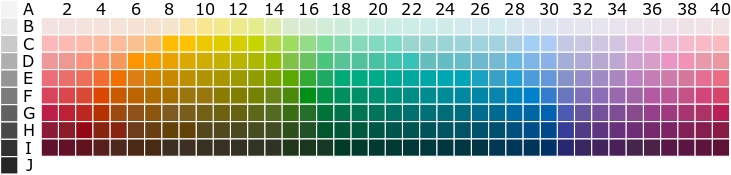
\includegraphics[width=.9\textwidth]{image/analysis/munsell_o.png}
\caption{Munsell 330 Colour Chip}
\label{fig:munsell_ori330}
\end{figure}


\begin{comment}
\begin{figure}[htb!]
  \centering
\begin{tabular}{cc}
 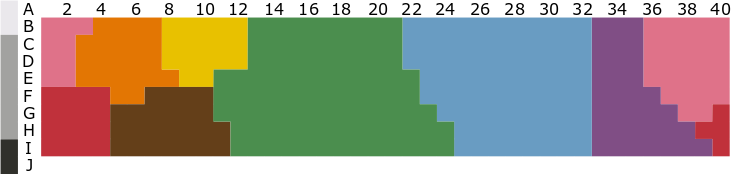
\includegraphics[width=0.45\linewidth]{image/analysis/munsell_a.png}   &
 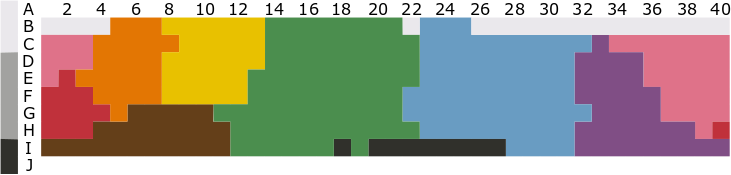
\includegraphics[width=0.45\linewidth]{image/analysis/munsell_b.png}   \\
(a) Parametric model &
(b) PLSA-individual  \\
 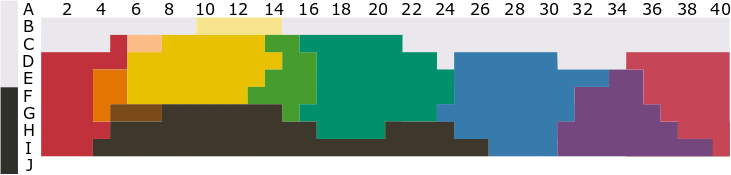
\includegraphics[width=0.45\linewidth]{image/analysis/munsell_e.png}  &
 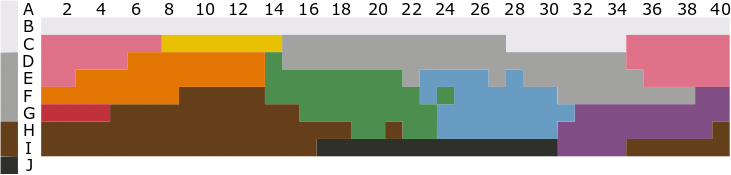
\includegraphics[width=0.45\linewidth]{image/analysis/munsell_d.png}   \\
(c) Linguistic Approach &
(d) Our method \\
\end{tabular}
\caption[Comparison of the Munsell 330 Colour Chips and the Assigned Colour Terms]{Comparison of the Munsell 330 Colour Chips and the Assigned Colour Terms. (a) Parametric model. Image reproduced from \citeA{benavente2008parametric}; (b) PLSA-individual. Image reproduced from \citeA{van2009learning}; (c) Linguistic Approach. Image reproduced from \citeA{zaslavsky2018efficient}; (d) Proposed Method } \label{fig:munsell_compare}
\end{figure}
\end{comment}



\begin{figure}[htb!]
  \centering
\begin{tabular}{c}
 (a) Parametric model \\
 \includegraphics[width=0.7\linewidth]{image/analysis/munsell_a.png}   \\
 (b) PLSA-individual  \\
 \includegraphics[width=0.7\linewidth]{image/analysis/munsell_b.png}   \\
 (c) Linguistic Approach, Before Compression \\
 \includegraphics[width=0.7\linewidth]{image/analysis/munsell_c.png}   \\
 (d) Linguistic Approach, After Compression \\
 \includegraphics[width=0.7\linewidth]{image/analysis/munsell_e.png}  \\
 (e) Proposed method\\
 \includegraphics[width=0.7\linewidth]{image/analysis/munsell_d.png}   \\
\end{tabular}
\caption[Comparison of the Munsell 330 Colour Chips and the Assigned Colour Terms]{Comparison of the Munsell 330 Colour Chips and the Assigned Colour Terms. (a) Parametric model. Image reproduced from \citeA{benavente2008parametric}; (b) PLSA-individual. Image reproduced from \citeA{van2009learning}; (c, d) Linguistic Approach (Before \& After compression). Image reproduced from \citeA{zaslavsky2018efficient}; (e) Proposed Method } \label{fig:munsell_compare}
\end{figure}


\begin{table}[H]\centering
\begin{tabular}{|l|c|c|}
\hline
\textbf{Method}                             & \textbf{\# of votes} & \textbf{Percentage (\%)} \\ \hline
(a) Parametric model                        & 17                   & 22.08              \\ \hline
(b) PLSA-individual                         & 20                   & 25.97              \\ \hline
(c) Linguistic Approach, Before Compression & 4                    & 5.19              \\ \hline
(d) Linguistic Approach, After Compression  & 24                   & 31.17              \\ \hline
(e) Proposed method                         & 12                   & 15.58              \\ \hline
\end{tabular}
\caption{User study: Understanding Users' Preference on How Colour Terms Should Be Allocated}
\label{tab:munsell_result}
\end{table}

\vspace{-2em}




\subsection{Motion Semantic Extraction}
\label{subsec:chamferdistancemotionextraction}

With the intention of extracting motion information from the input video data, the spatio-temporal cuboids or \emph{atoms} were adopted here. Contrary to the framework used in \versionOneExt's motion extraction framework, instead of grouping the motions into 9 directional bins, only the location information of the vehicle at each frame is extracted. This eliminates the use of handcrafted parameters while ensuring important low-level semantics are stored while remaining its ability to represent motion information.


\begin{equation}
\label{eq:centroid}
(Centroid_x, Centroid_y) = (\frac{BB_{x}+BB_{width}}{2} , \frac{BB_{y}+BB_{height}}{2})
\end{equation}
\vspace{-2em}
\begin{align*}
    \text{where BB is the Bounding Box of the vehicle}
\end{align*}

As the background subtraction method has identified the vehicle's location, the centroid of the vehicle can be easily computed by inferring the data from bounding box using Equation~\ref{eq:centroid}. Using the \emph{atoms} structure as introduced in Section~\ref{section:framework}, each \emph{atom} can be uniquely identified using its' respective identifier via its x, y, and t-coordinate. A vehicle's trajectory, $P$, can be denoted using the collection of vehicle's centroid from each tracked frame in its life cycle. In this framework, the exact motion of the vehicle held lesser importance when compared to the locality of the vehicle itself.

\begin{align}
    P &= \{ (x_i, y_i, t_i), (x_{i+1}, y_{i+1}, t_{i+1}), (x_{i+2}, y_{i+2}, t_{i+2}), \dotsb,(x_{i+n}, y_{i+n}, t_{i+n})\}  \nonumber \\
      &= \{ t_{p1}, t_{p2}, t_{p3}, \dotsb, t_{pn}\}
\end{align}


To determine the motion of the vehicle, the sequence of the centroids' t-coordinates are used to represents the motion and the trajectory, $P$, of a vehicle. Figure~\ref{fig:motionExample} illustrates the property of this setup which allows trajectories of vehicles to be identified only using the centroid information. Upon obtaining the location of the centroids, the x \& y-coordinate can be inferred as the atom's width and heights were predefined. Finally, the sequence of the t-coordinate along with the x \& y-coordinates are written into the database as a means of collecting motion information.

\begin{figure}[hbt!]\centering
\includegraphics[width=.9\textwidth]{image/general/trajectorysample2.png}
\caption{Collection of a Vehicle's Centroid to Represent the Vehicle's Motion}
\label{fig:motionExample}
\end{figure}

As a vehicle in the car park scene generally does not move in an irregular motion, the sequence information of the vehicle's centroid holds sufficient clue for the reconstruction and estimation of a vehicle's trajectory within the car park scene. This setup also allows reduction of overhead computational cost and storage space which might occur when converting these centroid information into finer vector features.

\section{Summary}
In this chapter, two different semantic extraction methods are proposed. The extracted semantics includes the time-date information, colour, motion, object type as well as the size of the objects. Both methods employed slightly different methods of extracting the colour and motion information, the performance of these proposed methods will be discussed in Section~\ref{section:retrievalengine}.

In comparison with the existing methods of extracting vehicle colour semantics described in Section~\ref{section:litreview}, the proposed method in this work is able to extract vehicle colour information from videos with relatively low resolution.
Furthermore, analysis was done to compare the results obtained using methods proposed in \versionOneExt and \versionTwoExt. The analysis on several colour term mapping methods against the WCS stimulus palette was also studied to better understand the advantage and disadvantages of the proposed method.

The analysis shows that both proposed methods drastically decrease in performance if the entire vehicle is occluded or when vehicles are in the shadow. Likewise, the extraction of dominant colour fails when dealing with multi-coloured vehicles.
Furthermore, as the mapping of colour terms are subjective to each individual, a user study was performed. The tabulated results show that most users prefer the colour model proposed by \citeA{zaslavsky2018efficient} after compression.
In the future, the colour term mapping function can be potentially improved so that the results would resemble the best colour mapping function.

